\documentclass{beamer}

\usepackage{beamerthemesplit}
\usepackage{color}
\usepackage{listings}
\usepackage[cache=false,outputdir=.texpadtmp]{minted}

\lstset{
	backgroundcolor=\color{white},
	tabsize=4,
	rulecolor=\color{blue},
	language=Haskell,
        basicstyle=\scriptsize,
        upquote=true,
        aboveskip={1.5\baselineskip},
        columns=fixed,
        showstringspaces=false,
        extendedchars=true,
        breaklines=true,
        prebreak = \raisebox{0ex}[0ex][0ex]{\ensuremath{\hookleftarrow}},
        frame=single,
        showtabs=false,
        showspaces=false,
        showstringspaces=false,
        identifierstyle=\color[rgb]{0,0.7,0.7},
        keywordstyle=\color[rgb]{0.7,0,0.7},
        commentstyle=\color[rgb]{1,0,0},
        stringstyle=\color[rgb]{0.4,0.4,0.4},
		upquote=false
}

\begin{document}


\begin{frame}
    \frametitle{Rapid Prototyping With Coconut}

	{\bf COCONUT}: ({\bf CO}de {\bf CON}structing {\bf U}ser {\bf T}ool) \\
	\begin{itemize}
	    \item An embedded DSL in Haskell for simulating and generating assembly code
	\end{itemize}

    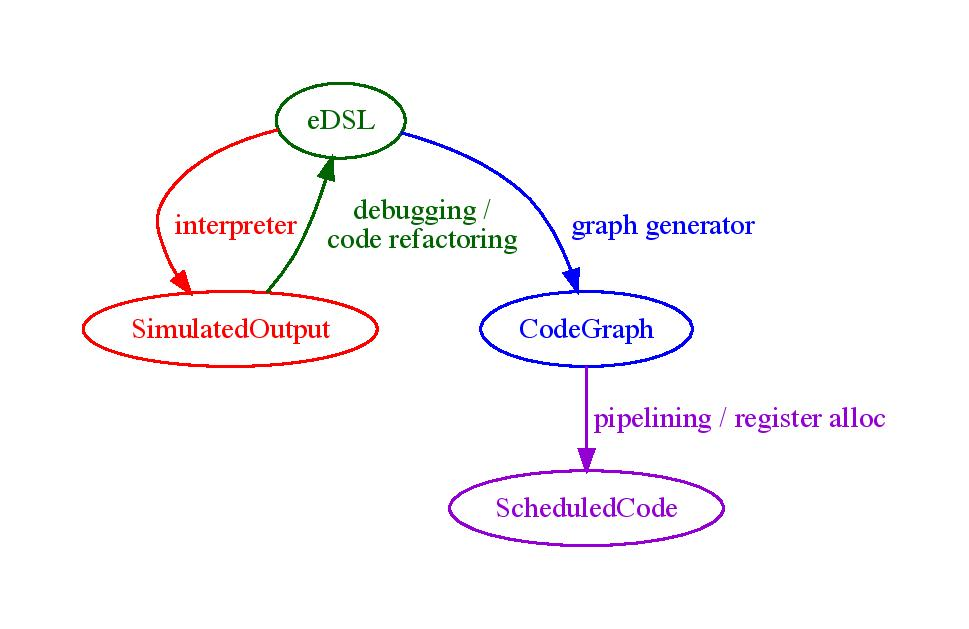
\includegraphics[scale=0.5]{prototyping.pdf}
\end{frame}      

\begin{frame}[fragile]
    \frametitle{Rapid Prototyping With Coconut}
    
    The Coconut {\bf Domain Specific Language} allows the embedding of assembly code in 
    \qquad \\
        \begin{itemize}
            \item a {\bf type safe}, high level language (Haskell)
            \item without consideration for {\bf register allocation / pipelining}
            \item allows simulation of both scheduled and unscheduled code
            \item allows fine tuning of optimizations applied to generated code graphs
        \end{itemize}    
\end{frame}

\begin{frame}[fragile]
    \frametitle{Rapid Prototyping With Coconut}

\begin{itemize}
    \item {\color{blue} Example:} Inlined Assembly Code \\
    \qquad \\
\begin{minted}{haskell}
#define INLINED_CODE(a0,b0,c0,..) \ 
vadd a0,b0,a0 \   
vsub a0,c0,a0 \  
...          
\end{minted}

    \item {\color{blue} Example:} Corresponding Haskell Embedded Coconut Code \\
    \qquad \\
\begin{minted}{haskell}                                 
inlined_code (a0,b0,c0,...) = let
    a0_0 = vadd b0 a0
    a0_1 = vsub c0 a0_0
    ...
   in [a0_0,a0_1,...]                          
\end{minted}
\end{itemize}
\end{frame}

\begin{frame}[fragile]
    \frametitle{Relaxed Continous Optimization based Instruction Scheduling}   
    Per Instruction $i$, perform a relaxation of scheduled position to dispatch and completion times $t_i$, $b_i$
    \begin{align*}
    \text{\color{cyan} Objective Variables \qquad} & t_i, b_i, f_i:& \mathbb{R} \\
    \text{\color{cyan} Constants \qquad} & \textrm{II} :& \mathbb{R} \\
    \text{\color{cyan} Indicator Function \qquad} & \mathsf{IN} :& \mathbb{R} \rightarrow \mathbb{R} \\
    & t_i :& \text{dispatch time} \\
    & b_i :& \text{completion time} \\
    & f_i :& \text{FIFO use } 0 \leq f_i \leq 1 \\
    & \textrm{II} :& \text{iteration interval} \frac{\# instructions}{dispatches/cycle} \\
    \end{align*}
\end{frame}

\end{document}
